\section{Method}

In order to develop models and test hypotheses, it was necessary to establish a significant corpus of brainstorming data data. Over the course of four months we repeatedly collected responses to brainstorming tasks.

Participants were recruited from Amazon's \emph{Mechanical Turk} \cite{_amazon_????}, and were restricted to residents of the United States for a baseline expectation of english language comprehension and cultural familiarity. Mechanical Turk is an online marketplace in which members receive financial reward for completing \emph{Human Intelligence Tasks}, or HITs.

HITs were placed on the marketplace asking for a variable \emph{number of ideas}, with proportional rewards. These conditions were : 5 ideas (with a corresponding reward of \$0.18 USD), 10 ideas (\$0.35), 20 (\$0.70), 50 (\$1.75), 75 (\$2.65), and 100 (\$3.50).

This served as the independent variable in all data gathering. It must be stated that under normal brainstorming conditions, participants are asked to generate as many ideas as possible within a fixed time frame, instead of a fixed number. We excluded such a condition for two reasons. First, it is practice in crowd creativity tasks to solicit a fixed number of ideas (e.g. Yu and Nickerson \cite{yu_cooks_2011}). Secondly, we piloted asking respondants for "as many ideas as possible" in a generous time frame. Over N respondents, we received a mean of N ideas (std N), despite giving a financial of \$\$\$\$. This suggested a propensity to "game the system", a behaviour we wanted to exclude.

While the brainstorming question was manipulated in pilot studies, it was fixed for the data reported on in this paper:

\begin{itemize}
\item \textbf{MP3}

Many people have old MP3 players or MP3 players that they no longer use. Please brainstorm N uses for old MP3 players/MP3 players. Assume that the devices' batteries no longer work, though they can be powered via external power sources. Also be aware that devices may \emph{not} have displays. Be as specific as possible in your descriptions.
\end{itemize}

This problem was selected for three qualities:

\begin{enumerate}
\item It requires creativity to resolve. Obvious answers do not satisfy the problem.
\item Mechanical Turk participants have the expertise to solve the problem.
\item It has an associated success metric.
\end{enumerate}

Workers choose which \emph{number of ideas} condition to participate in, thus self-selection bias is a reasonable concern. However, this bias is also present in real-world HIT choice behaviour. 

Upon accepting a HIT, participants were asked to give consent and informed that they could leave the study at any point without financial consequences. Under normal conditions, the participants would be expected to complete all responses to receive compensation.

Should we be dropping these runs, or at least testing they don't have an affect?

\subsection{Task}

The brainstorming task is a form in a standard web browser. Participants are presented with a brief overview of the tenets of brainstorming, are presented a problem, and must enter some number of ideas to resolve the problem within an 18 hour period.

At the beginning of the form is a brief introduction to brainstorming, with a paraphrase of Osborne's four rules of brainstorming \cite{osborn_applied_1957}. These rules were manipulated to make sense within the constraints nominal brainstorming over the web medium. The rules, as displayed to the participants:

\begin{enumerate}
\item There are no bad ideas. Don't criticise your choices.
\item Wild ideas and building off of old ideas are okay.
\item Quantity of ideas is prioritized.
\item Combinations of ideas count as new ideas.
\end{enumerate}

The brainstorming problem is below this, followed by a series of text entry inputs numbered through to the total number of ideas requested. Figure X (FIG) is an example of a typical task. We place a larger free text area at the bottom of the list where participants could enter any additional ideas.

\subsubsection{Data Collected}

In total, 161 HITs were complteed by 146 distinct participants, for a total of 3007 responses. A breakdown of responses across conditions is given in table TAB. In cases when a single participant participated in multiple conditions, all HITs after the first were dropped for subsequent analysis.

\begin{tabular}[h!]{r | l l l l l l }
& 5 & 10 & 20 & 50 & 75 & 100 \\ \hline \hline
HITs completed & 59 & 49 & 23 & 10 & 10 & 10 \\
HITs completed (no repeats) & 57 & 39 & 21 & 9 & 10 & 10 \\
solutions (no repeats) & 283 & 372 & 413 & 450 & 635 & 855 \\
\end{tabular}

HITs were augmented with JavaScript to collect data in addition to brainstorming responses. For each response, we collected the time of the first activation and last de-activation of the corresponding form element. We collected the time the HIT was accepted and the time it was submitted. To uniquely identify participants, we computed a hash of their Mechanical Turk worker ID. A hash was used to protect privacy after data release.

\subsection{Terminology}

To facilitate discussion, we introduce terms here that we will use throughout the rest of the paper.

An \emph{instance} is a single solution by a single participant to a brainstorming question. Alternatively, an instance may be thought of as the text entered into a single field in the task form. For example, figure~\ref{fig:sample_instances} gives four \emph{instances} from the data set.

\begin{figure}[!h]
    \begin{enumerate}
        \item "Storage Container"
        \item "Small Storage Box"
        \item "Coin Storage"
        \item "Travel Jewelry Case"
    \end{enumerate}
    \label{sample_instances}
\end{figure}

A \emph{brainstorming run}, or \emph{run}, is the temporally-ordered series of instances that were received in a single HIT by a single user. As stated above, after dropping repeat data, all brainstorming runs were completed by distinct participants.

An \emph{idea} is a unique solution to the brainstorming problem. An instance is associated with exactly one \emph{idea}, and all instances in the same idea should be paraphrases of one another. In Figure FIG, "Storage Container" and "Small Storage Box" belong to the same \emph{idea}. However, "Coin Storage" does not belong to the same idea, as it contains additional information.

Despite this, it is clear the ideas have some commonality. It is desireable to encode this relationship. To that end, we propose a hierarchical clustering of ideas in \emph{category trees}. In a category tree, ideas act as nodes. Each idea may have 0 or 1 parent idea (only the root has 0) and 0 or more child ideas. An example category tree for the instances in Figure FIG is given in Figure FIG.

\begin{figure}[!h]
    \centering
    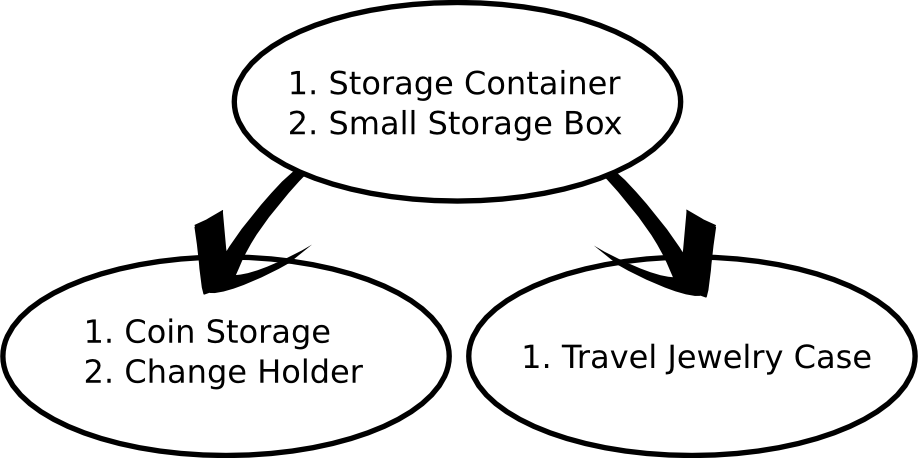
\includegraphics[width=0.9\columnwidth]{example_instances}
\end{figure}

If an idea \emph{A} is a parent of idea \emph{B}, A is a generalization of B: all instances in A are are suitably general to encompass all instances in B. This hierarchical clustering allows us to classify ideas as simultaneously different in solution stragy but different in solution details.

We further distinguish category trees into \emph{singleton} and \emph{non-singleton} category trees. A singleton category tree is composed of only one idea node, the root. A non-singleton category tree has at least two idea nodes. We introduce non-singleton category trees as correspondents to the images in Nisjstad and Stroebe's SIAM model \cite{nijstad_how_2006}. On SIAM, the idea generation process is represented by a series of images activations within which idea production occurs. Non-singleton trees by definition represent strategies that have been produced in at least two distinct ways.

The \emph{idea forest} is the collection of all category trees. Different trees in the forest have no particular relationship.

\subsection{Clustering}

In addition to the notion of an idea forest, we also propose a clustering algorithm driven by human intelligence to create the data structure. The algorithm is described in Figure~\ref{fig:cluseringalg}. Instances are added one at a time to the existing idea forest. In brief summary, the root idea that most closely matches the strategy in the instance is selected, and then that root idea and the new instance are compared in generality. This process may be repeated depending on this generality relationship, until instance is either placed in an existing idea or a new idea node is created.

\begin{figure*}[ht]
\small
\begin{verbatim}
for each instance:
  idea_node = new node including instance
  current_node = root of forest
  do:
    best_match = max_similarity(idea_node, current_node.children)

    if best_match.similarity is low or current_node has no children:
      insert idea_node under current_node
      exit do
    else:
      if coverage(idea_node, best_match) == coverage(best_match, idea_node) == high:
        merge idea_node, best_match
        exit do
      else if coverage(idea_node, best_match) == coverage(best_match, idea_node) == low:
        new_parent = new artifical idea node
        insert best_match, idea_node under new_parent
        insert new_parent under current_node
        exit do
      else if coverage(idea_node, best_match) > coverage(best_match, idea_node):
        replace best_match with idea_node in tree
        current_node = idea_node
        idea_node = best_match
      else:
        current_node = best_match
\end{verbatim}
\caption{Manual clustering algorithm}
\label{fig:cluseringalg}
\end{figure*}

The clustering algorithm relies on the human intelligence of the researcher for three key decisions:

\subsubsection{Similarity}
Two nodes a and b have high similarity if they solve the problem in the same way, and low similarity if their solutions have no common themes. For example, in Figure FIG, "Small Storage Box" and "Travel Jewelry Case" have high similarity, as they both solve the problem of using a broken MP3 player by using it to reflect light.

\subsubsection{Coverage}
A node a has high coverage of a node b if the problem solution in a is equal to or an abstraction of the problem solution in b. Coverage is not commutative. To return to the example, "Small Storage Box" has high coverage of "Travel Jewelry Case", as the latter is a just a specific use for the former. On the other hand, the latter idea has low coverage of the former.

\subsubsection{Artificial Ideas}
Occasionally, two nodes have high similarity but no coverage. For example, "Coin Storage" and "Travel Jewelry Case" use the MP3 player in the same way, but neither is a generalization of the other. In this case, the algorithm appeals to the human coder to provide a lable for a new idea that is a generalization of both.

The primary author followed the algorithm to cluster the 3007 response instances into ideas and trees.
